\section{Auswertung und Diskussion}
\label{sec:AuswertungDiskussion}

\subsection*{Bestrahlungsplan für das PTV-Intermediate}

In den Abbildungen \ref{abb:Z1}, \ref{abb:Y1} und \ref{abb:X1} ist die resultierende Dosisverteilung
in unterschiedlichen Ansichten dargestellt. Dabei ist
zu sehen, dass es nicht gelungen ist das gesamte PTV-Intermediate mit der $95\%$ Isodosenlinie zu umschließen.
Das liegt daran, da das PTV sehr nah an die Blase und an das Rektum heranreicht und diese Organe Risikoorgane sind.
Da bei dieser Bestrahlung eine relativ große Dosis appliziert wird, müssen die Risikoorgane ausreichend geschont werden, damit die
Organdosisgrenzwerte nicht überschritten werden. Die maximale relative Dosis bei dieser Bestrahlung beträgt $107,7\%$ und wird außerhalb des PTVs
deponiert. Da allerdings die maximale relative Dosis innerhalb des PTVs bei $107,6\%$ liegt, wird die maximale Dosis im Rumpf sehr nah an dem PTV deponiert
und auch nur an ein sehr geringes Volumen außerhalb des PTVs. Die maximale relative Dosis liegt minimal oberhalb der erlaubten maximalen Dosis von
$107\%$ \cite{ICRU}. Die minimale Dosis innerhalb des PTVs liegt bei $81,1\%$, was unterhalb der gewünschten minimalen Dosis von $95\%$ liegt.
Das konnte auch schon anhand der Dosisverteilung gesehen werden, dass vor allem in Bereichen des PTVs, die nah an den Risikoorganen
liegen, eine relative Dosis von $95\%$ nicht erreicht werden konnte.


\begin{figure}[H]
  \centering
  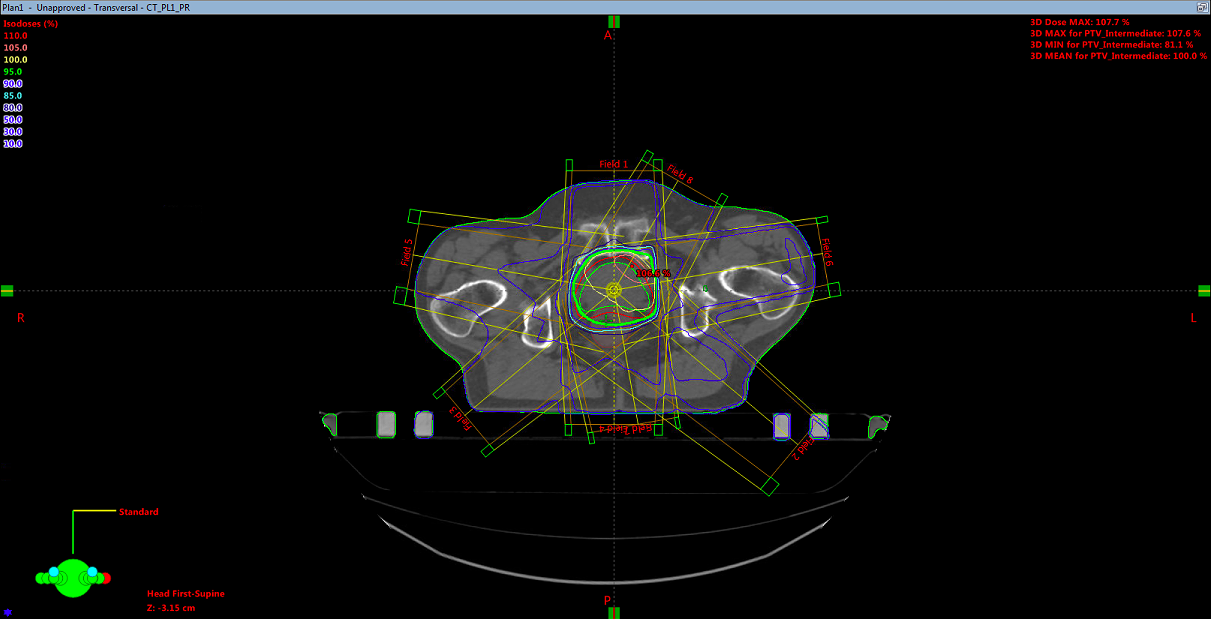
\includegraphics[width=\textwidth]{Bilder/Prostata1_Z.png}
  \caption{Darstellung der Dosisverteilung im Rumpf in Transversalansicht.}
  \label{abb:Z1}
\end{figure}

\begin{figure}[H]
  \centering
  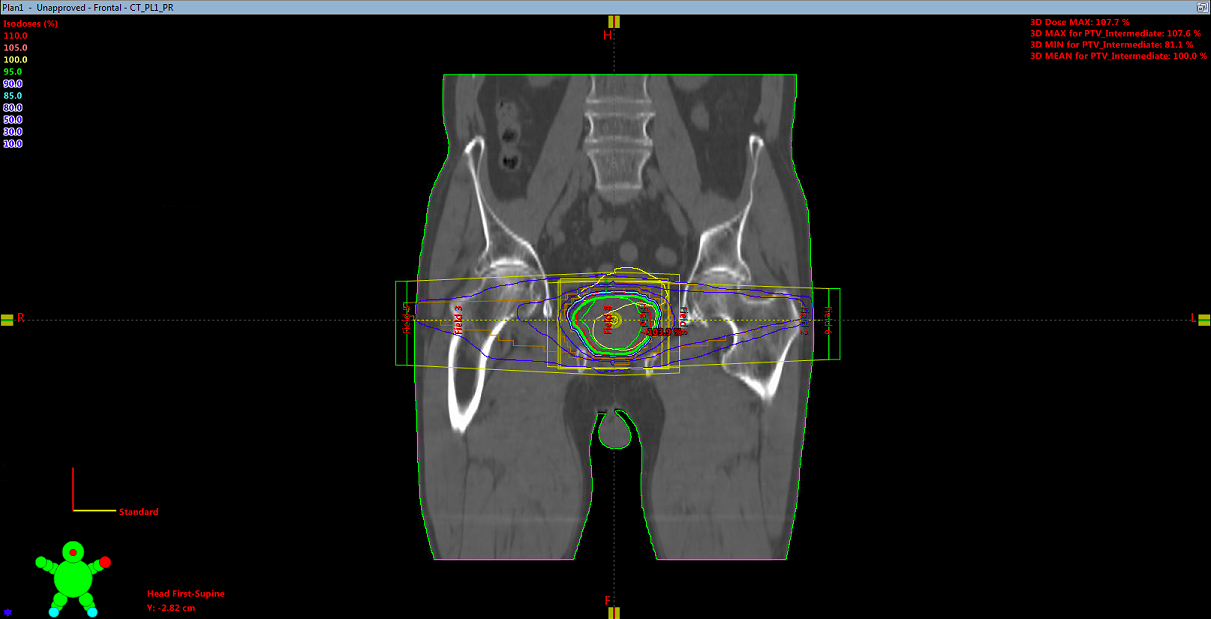
\includegraphics[width=\textwidth]{Bilder/Prostata1_Y.png}
  \caption{Darstellung der Dosisverteilung im Rumpf in Frontalansicht.}
  \label{abb:Y1}
\end{figure}

\begin{figure}[H]
  \centering
  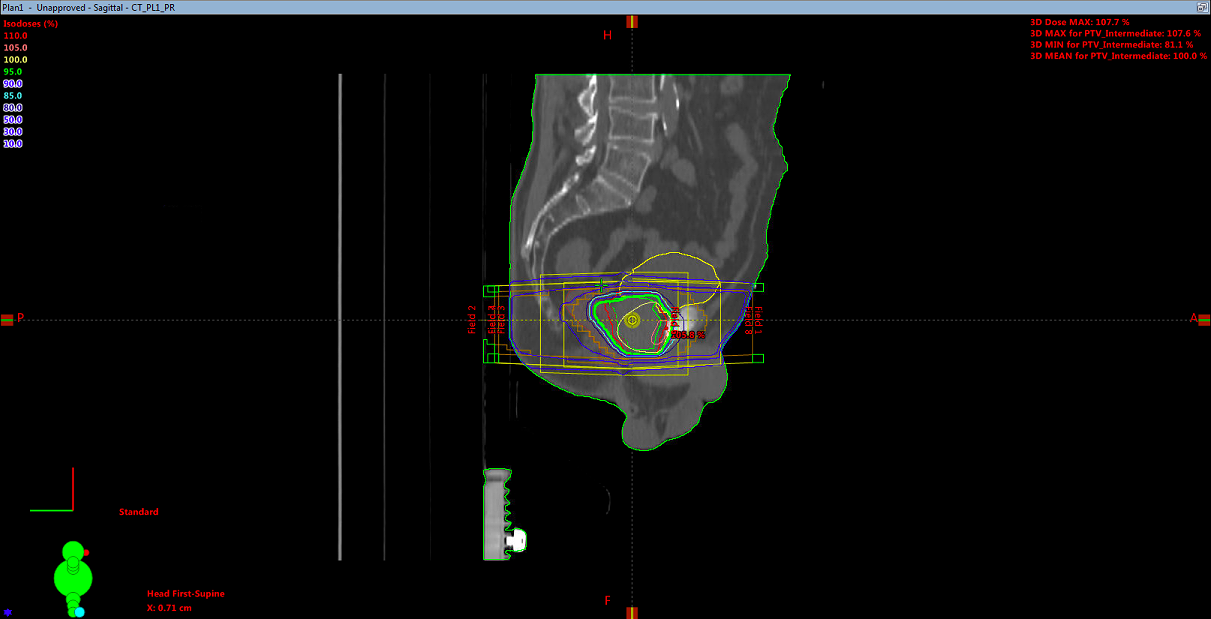
\includegraphics[width=\textwidth]{Bilder/Prostata1_X.png}
  \caption{Darstellung der Dosisverteilung im Rumpf in Sagittalansicht.}
  \label{abb:X1}
\end{figure}

Für eine bessere Beurteilung der Dosisverteilung ist das DVH dieser Bestrahlung in der
Abbildung \ref{abb:DVH1} dargestellt. Dabei ist anhand der DVH Kurve des PTV-Intermediates
(rot) zu erkennen, dass noch etwa $92\%$ des PTVs noch eine relative Dosis von $95\%$ erhält.
Allerdings ist zu erkennen, dass die meisten Risikoorgane gut geschont werden konnten, da
die DVH Kurven der Hüftköpfe und der Blase schnell abfallen. Nur das Rektum und der Dünndarm konnten bei
diesem Bestrahlungsplan nicht gut geschont werden. Um zu überprüfen ob die Organdosisgrenzwerte
eingehalten worden sind, werden beide Bestrahlungspläne am Ende zusammen betrachtet.

\begin{figure}[H]
  \centering
  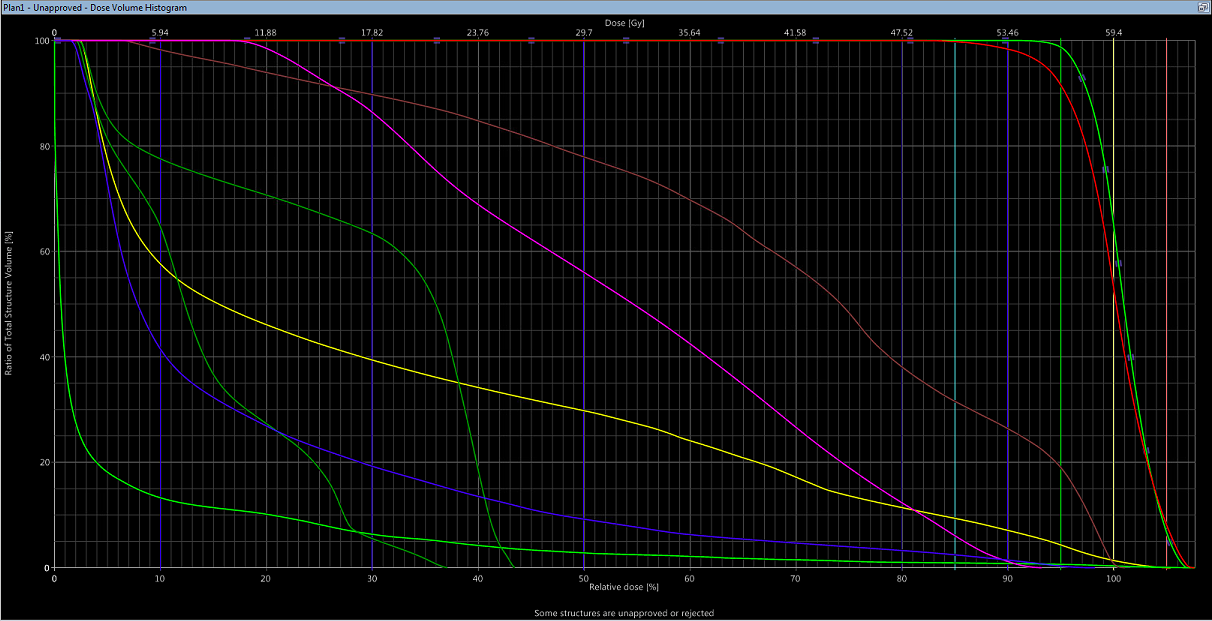
\includegraphics[width=\textwidth]{Bilder/Prostata1_DVH.png}
  \caption{Dosis-Volumen-Histogramm für das PTV-Intermediate in rot und den gesamten Rumpf in grün. Außerdem ist das DVH für das Blase in gelb, für den linken Hüftkopf in hellgrün, für den rechten Hüftkopf in dunkelgrün, für das Rektum in braun, für den Darmbeutel in Blau, für den Dünndarm in lila und für die Prostata in grün dargestellt.}
  \label{abb:DVH1}
\end{figure}


\subsection*{Bestrahlungsplan für das PTV-High}

Bei dem zweiten Bestrahlungsplan wird das PTV-High bestrahlt. Die sich ergebene Dosisverteilung
ist in den Abbildungen \ref{abb:Z2}, \ref{abb:Y2} und \ref{abb:X2} in verschiedenen
Ansichten dargestellt. Auch bei dieser Bestrahlung ist es nicht gelungen das PTV komplett
mit der $95\%$ Isodosenlinie zu umschließen. Das kommt daher, dass auch das PTV-High in der
Mitte von den Risikoorganen liegt und es musste darauf geachtet werden, dass diese Organe hinreichend
gut geschont werden. Aus diesem Grund ist die minimale relative Dosis innerhalb des PTVs
$79,6\%$. Die maximale relative Dosis wird außerhalb des PTVs deponiert und liegt
bei $115,7\%$. Allerdings wird diese Dosis nicht in dem Patienten deponiert, sondern einem
Teil der Patientenliege, die als Body konturiert worden ist (siehe Abbildung \ref{abb:Z2}).
Anhand der Dosisverteilung ist zu erkennen, dass die relative maximale Dosis, die in dem
Patienten deponiert wird, in dem PTV deponiert wird. Dort ist die maximale relative Dosis
$106,9\%$ und diese Dosis liegt unterhalb der erlaubten maximalen Dosis.

\begin{figure}[H]
  \centering
  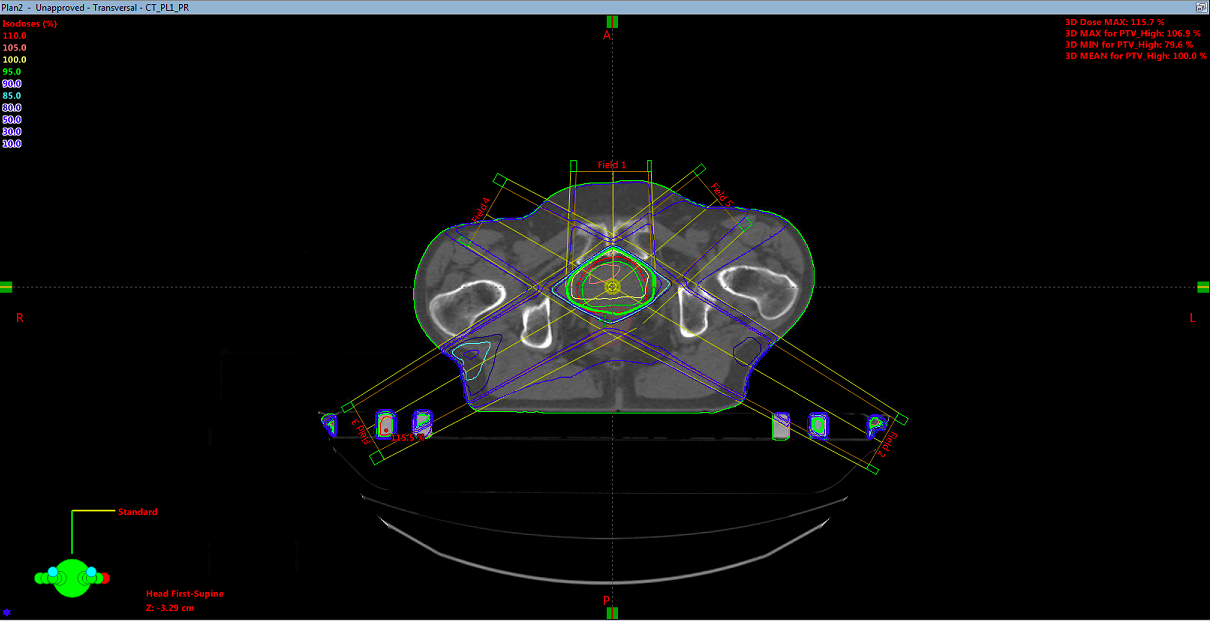
\includegraphics[width=\textwidth]{Bilder/Prostata2_Z.png}
  \caption{Darstellung der Dosisverteilung im Rumpf in Transversalansicht.}
  \label{abb:Z2}
\end{figure}

\begin{figure}[H]
  \centering
  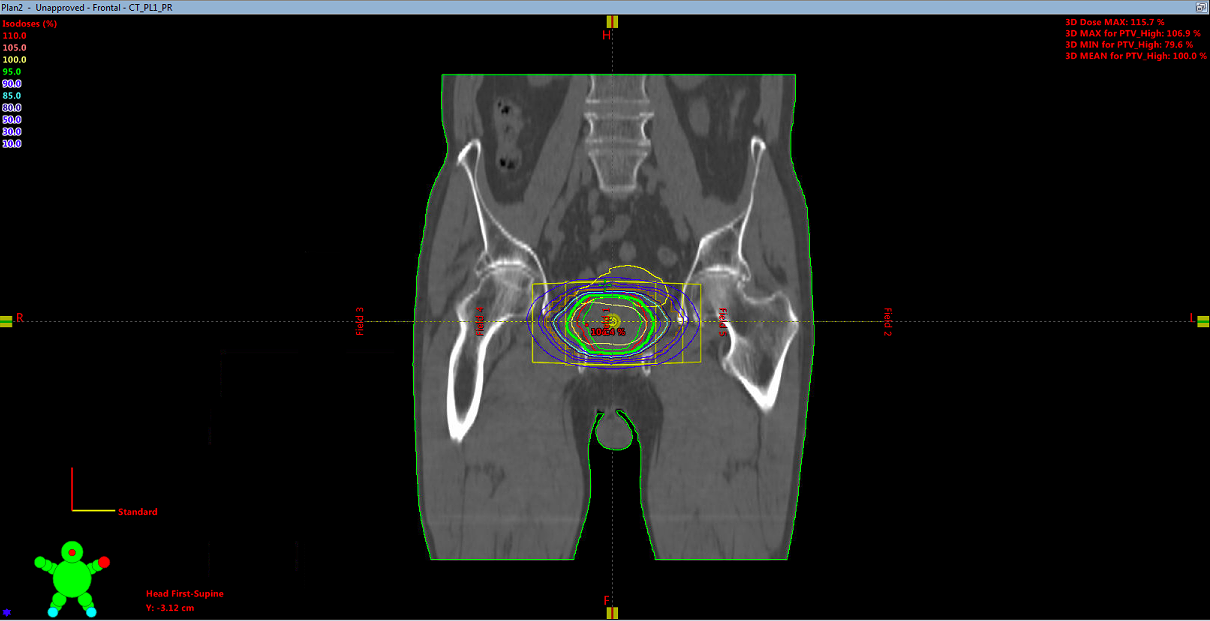
\includegraphics[width=\textwidth]{Bilder/Prostata2_Y.png}
  \caption{Darstellung der Dosisverteilung im Rumpf in Frontalansicht.}
  \label{abb:Y2}
\end{figure}

\begin{figure}[H]
  \centering
  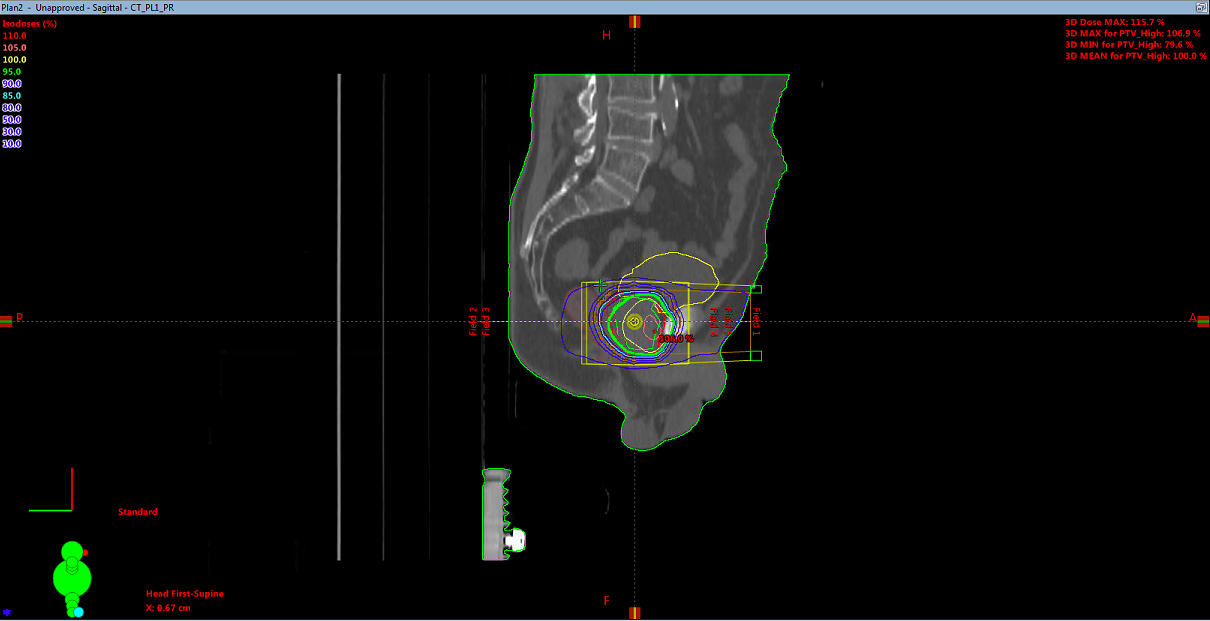
\includegraphics[width=\textwidth]{Bilder/Prostata2_X.png}
  \caption{Darstellung der Dosisverteilung im Rumpf in Sagittalansicht.}
  \label{abb:X2}
\end{figure}

Auch bei diesen Bestrahlungsplan wird ein DVH erzeugt, welches in der Abbildung \ref{abb:DVH2}
dargestellt ist. Dabei ist anhand der DVH Kurve des PTVs (rot) zu erkennen, dass etwa $90\%$ des
PTVs mit der $95\%$ Isodosenlinie umschlossen werden konnte. Auch bei diesem
Bestrahlungsplan kommt das daher, da sich viele Risikoorgane in unmittelbarer Nähe zu dem
PTV befinden. Anhand der DVH Kurven der Risikoorgane ist gut zu sehen, dass es gelungen ist diese
Organe zu schonen.

\begin{figure}[H]
  \centering
  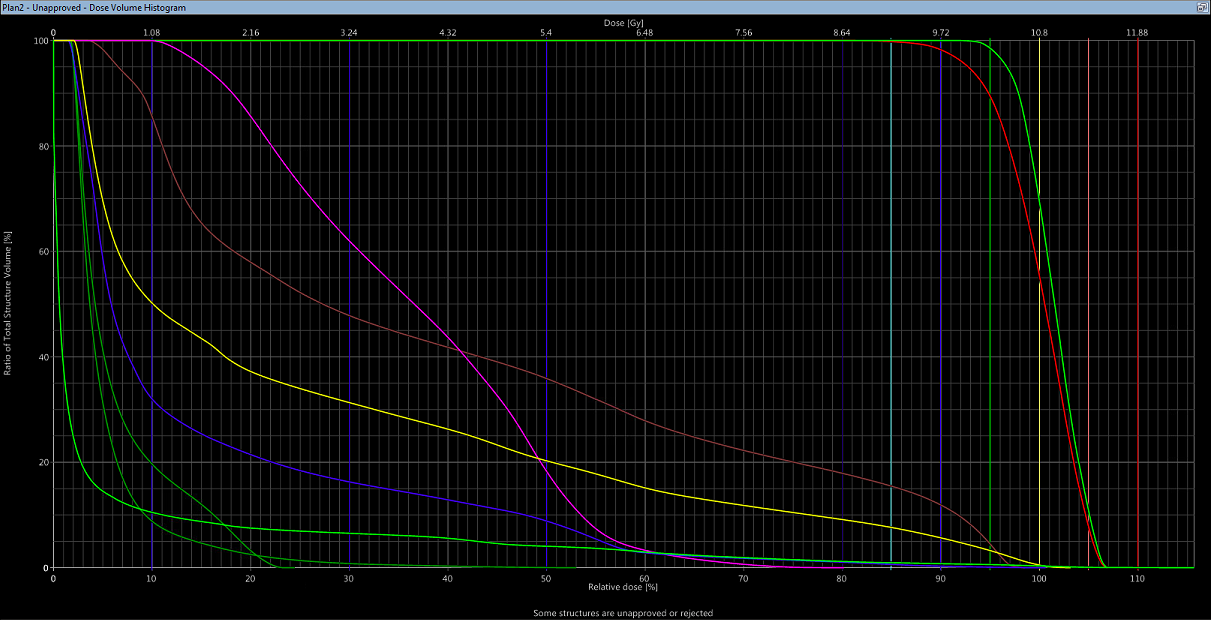
\includegraphics[width=\textwidth]{Bilder/Prostata2_DVH.png}
  \caption{Dosis-Volumen-Histogramm für das PTV-High in rot und den gesamten Rumpf in grün. Außerdem ist das DVH für das Blase in gelb, für den linken Hüftkopf in hellgrün, für den rechten Hüftkopf in dunkelgrün, für das Rektum in braun, für den Darmbeutel in Blau, für den Dünndarm in lila und für die Prostata in grün dargestellt.}
  \label{abb:DVH2}
\end{figure}


\subsubsection*{Summe der Bestrahlungspläne}

Für die Beurteilung, ob die Organdosisgrenzwerte der Risikoorgane eingehalten worden sind,
wird ein DVH der Summe der beiden Bestrahlungspläne erzeugt. Dieses ist in der Abbildung
\ref{abb:DVHsum} gezeigt. Für das Rektum ist vorgeschrieben, dass
weniger als $50\%$ des Volumens des Rektums eine Dosis von $\SI{50}{\gray}$ erhalten darf und weniger als $35\%$
des Volumens eine Dosis von $\SI{60}{\gray}$ \cite{QUANTEC}. Für höhere Dosiswerte gibt es weitere Grenzwerte, die alle allerdings auch
eingehalten worden sind. Etwa $43\%$ des Volumens des Rektums erhält eine Dosis von $\SI{50}{\gray}$ und etwa $26\%$ des Volumens erhält noch eine
Dosis von $\SI{60}{\gray}$.
Bei der Blase ist bei einem Prostatakarzinom vorgeschrieben, dass weniger als $50\%$ des Volumens eine Dosis von weniger als $\SI{65}{\gray}$
erhalten darf \cite{QUANTEC}. Auch dieser Grenzwert konnte eingehalten werden, da nur etwa $5\%$ des Volumens eine Dosis von $\SI{65}{\gray}$
erhält. Die Hüftköpfe darf nur maximal $10\%$ des Volumens eine Dosis von $\SI{52}{\gray}$ erhalten \cite{QUANTEC}. Auch das wurde eingehalten, da
die maximale Dosis der Hüftköpfe $\SI{28.1}{\gray}$ und $\SI{24.538}{\gray}$ beträgt.
Bei dem Dünndarm darf weniger als $\SI{120}{\milli\liter}$ eine Dosis von $\SI{15}{\gray}$ erhalten \cite{QUANTEC}. Da
bei dieser Bestrahlung nur $\SI{12.3}{\milli\liter}$ des Dünndarm betrachtet werden, wird auch dieser Grenzwert eingehalten.


\begin{figure}[H]
  \centering
  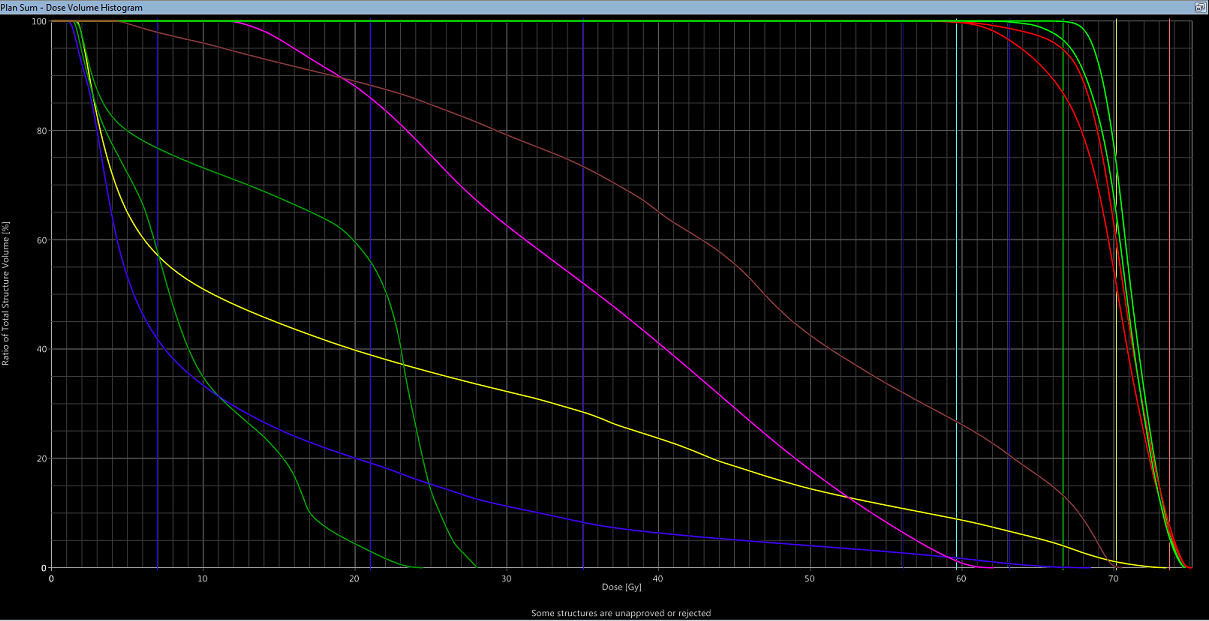
\includegraphics[width=\textwidth]{Bilder/DVHsum.png}
  \caption{Dosis-Volumen-Histogramm  für die Summe der Bestrahlungspläne. Dabei ist die DVH Kurven für die PTVs in rot dargestellt. Außerdem ist das DVH für das Blase in gelb, für den linken Hüftkopf in hellgrün, für den rechten Hüftkopf in dunkelgrün, für das Rektum in braun, für den Darmbeutel in Blau, für den Dünndarm in lila und für die Prostata in grün dargestellt.}
  \label{abb:DVHsum}
\end{figure}

Mit den erstellten Bestrahlungsplänen konnten die Zielvolumen zwar nicht komplett
mit der $95\%$ Isodosenlinie umschlossen werden, allerdings konnten alle Organdosisgrenzwerte
eingehalten werden. Da zumindest ein Großteil der Zielvolumina mit der gewünschten
Dosis versorgt werden konnten, sind die erstellten Bestrahlungspläne für diese Strahlentherapie gut geeignet.
